\section{Activities}
\begin{wrapfigure}{R}{0.3\textwidth}
\centering
\vspace{-10pt}
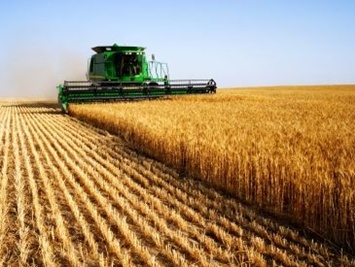
\includegraphics[width=0.3\textwidth, keepaspectratio]{images/pact/hoste}
\caption{\label{fig:activities}Picture of a combine harvester harvesting a field.}
\vspace{-10pt}
\end{wrapfigure}
In this chapter  the constraints and possibilities of the activity are presented, we are doing this to get a better overview of exactly this.
The purpose of the activity is to gain some form of overview of the resource usage when doing some form of work on a field.  This activity will happen ca. 4 times per field per year, which makes it somewhat frequent for some users and very infrequent for other users, relying on the amount of fields that the user interacts with. The activities are time sensitive, meaning you lose much of your produce if any of the tasks happen at a incorrect time. This time sensitivity may make the users more irritable due to the pressure they are under when doing the tasks. Due to this plausible irritability it should be easy to edit the input data, in case of any mistakes. This will be a abstract task that will require a user-friendly design, for proper usage. The input will be a considerable amount of data, which makes some form of keyboard almost required . 
